% Gemini theme
% https://github.com/anishathalye/gemini

\documentclass[final]{beamer}

% ====================
% Packages
% ====================

\usepackage[T1]{fontenc}
\usepackage{lmodern}
\usepackage[size=custom,width=120,height=72,scale=1.0]{beamerposter}
\usetheme{gemini}
\usecolortheme{gemini}
\usepackage{graphicx}
\usepackage{booktabs}
\usepackage{tikz}
\usepackage{pgfplots}
\usepackage{wrapfig}
\usepackage{subcaption}
\usepackage{mathtools}
\pgfplotsset{compat=1.17}
\graphicspath{{assets/}}

% ====================
% Lengths
% ====================

% If you have N columns, choose \sepwidth and \colwidth such that
% (N+1)*\sepwidth + N*\colwidth = \paperwidth
\newlength{\sepwidth}
\newlength{\colwidth}
\setlength{\sepwidth}{0.025\paperwidth}
\setlength{\colwidth}{0.3\paperwidth}

\newcommand{\separatorcolumn}{\begin{column}{\sepwidth}\end{column}}

% Logo
% \addtobeamertemplate{headline}{}
% {
%     \begin{tikzpicture}[remember picture,overlay]
%     \node [anchor=north east, inner sep=3cm] at ([xshift=1.4cm,yshift=1.3cm]current page.north east)
%       {\includegraphics[height=2.5cm]{assets/anl_logo.svg}};
%     \end{tikzpicture}
% }


% ====================
% Title
% ====================

\title{HMC with Normalizing Flows}
% \logoright{\includegraphics{assets/anl_logo.svg}}

\author{Sam Foreman\inst{1}, Taku Izubuchi\inst{2} Luchang Jin\inst{3}, Xiao-Yong Jin\inst{1}, James C. Osborn\inst{1},
Akio Tomiya\inst{3}}
% \author{Alyssa P. Hacker \inst{1} \and Ben Bitdiddle \inst{2} \and Lem E. Tweakit \inst{2}}

% \institute[shortinst]{\inst{1} Argonne National Laboratory \samelineand \inst{2} University of Connecticut}
\institute[shortinst]{\inst{1} Argonne National Laboratory \inst{2} RIKEN-BNL \inst{3} University of Connecticut}

% ====================
% Footer (optional)
% ====================

\footercontent{
  % \centering
  % The 38th International Symposium on Lattice Field Theory, 2021 \hspace*{\fill}
  % \separatorcolumn
  \href{https://github.com/nftqcd/fthmc}{github.com/nftqcd/fthmc} \hspace*{\fill}
  \separatorcolumn
  \href{mailto:foremans@anl.gov}{foremans@anl.gov}
}
% (can be left out to remove footer)

% ====================
% Logo (optional)
% ====================

% use this to include logos on the left and/or right side of the header:
% \logoright{\includegraphics[height=7cm]{logo1.pdf}}
% \logoleft{\includegraphics[height=7cm]{logo2.pdf}}

% ====================
% Body
% ====================

\begin{document}

\begin{frame}[t]
\begin{columns}[t]
\separatorcolumn

\begin{column}{\colwidth}

  \begin{block}{Normalizing Flows}
    For a random variable \(z\) with a given distribution \(z \sim r(z)\), and an invertible function \(x = f(z)\) with
    \(z = f^{-1}(x)\), we can use the change of variables formula to write
    %
    \begin{equation}
      p(x) = r(z)\left|\det{\frac{\partial z}{\partial x}}\right|
           = r{(f^{-1}(x))}\left|\det{\frac{\partial f^{-1}}{\partial x}}\right|
    \end{equation}
    %
    Where \(r(z)\) is the (simple) prior density, and our goal is to generate independent samples from the (difficult)
    target distribution \(p(x)\).
    %
    This can be done using \emph{normalizing flows} to construct a model density \(q(x)\) that approximates the target
    distribution, i.e. \(q(\cdot)\approx p(\cdot)\) for a suitably-chosen flow \(f\).
    %
    \begin{figure}%{r}{0.6\columnwidth}
      \includegraphics[width=0.66\columnwidth]{assets/flow_model6}
      \caption{\label{fig:flow_model}Using a Flow to generate data \(x'\). Image adapted from~\cite{weng2018flow}}
    \end{figure}

    We can construct a normalizing flow by composing multiple invertible functions \(f_{i}\) so that \(x\equiv [f_1\circ
    f_{2}\circ \cdots \circ f_{K}](z)\).
    %
    In practice, the functions \(f_{i}\) are usually implemented as \emph{coupling layers}, which update an ``active''
    subset of the variables, conditioned on the complimentary ``frozen'' variables.
    %
    % By sequentially updating alternating subsets of the variables in each coupling layer, we can ensure that all
    % variables are updated over the course of the flow.
    %
    \heading{Affine Coupling Layers}
    A particularly useful template function for constructing our normalizing flow is the affine coupling layer which is
    defined as 
    %
    \begin{align}
      f(x_{1}, x_{2}) &= \left(e^{s(x_{2})} x_{1} + t(x_{2}),\, x_{2}\right),%
        \quad\quad\text{with}\quad \log J(x) = \sum_{k}[s(x_{2})]_{k} \\
      f^{-1}(x'_{1}, x'_{2}) &= \left((x'_{1}-t(x'_{2}))e^{-s(x'_{2})},\, x'_{2}\right)%
        \quad\text{with}\quad \log J(x') = \sum_{k}-[s(x'_{2})]_{k}
    \end{align}
    %
    where \(s(x_{2})\) and \(t(x_{2})\) are of the same dimensionality as \(x_{1}\) and the functions act elementwise on
    the inputs.

    In order to effectively draw samples from the correct target distribution \(p(\cdot)\), our goal is to minimize the
    error introduced by approximating \(q(\cdot) \approx p(\cdot)\).
    %
    To do so, we use the (reverse) Kullback-Leibler (KL) divergence from Eq.~\ref{eq:kldiv}, which is minimized when \(p
    = q\).
    %
    \begin{equation}
      D_{\mathrm{KL}}(q||p) 
        \equiv \int dy\, q(y)[\log q(y) - \log p(y)]
        \approx \frac{1}{N} \sum_{i=1}^{N} \,[\log q(y_{i}) - \log p(y_{i})]\quad\text{where}\quad y_{i}\sim q.
        \label{eq:kldiv}
    \end{equation}
    % \begin{align}
    %   D_{\mathrm{KL}}(q||p)
    %     &\equiv \int dy\, q(y)[\log q(y) - \log p(y)]\\
    %     &\approx \frac{1}{N} \sum_{i=1}^{N} \,[\log q(y_{i}) - \log p(y_{i})]\quad\text{where}\quad y_{i}\sim q.
    %     \label{eq:kldiv}
    % \end{align}
    % We define the \emph{effective sample size} (ESS) for a batch of samples \(x_{i}\) as
    % %
    % \begin{equation}
    %   \mathrm{ESS} = \frac{\left(\frac{1}{N}\sum_{i} p(x_{i}) / q(x_{i})\right)^{2}}%
    %   {\frac{1}{N}\sum_{i}\left(p(x_{i})/q(x_{i})\right)^{2}} \in [0, 1],
    % \end{equation}
    % %
    % which provides a measure of correlations between samples in our batch, and a value of \(1\) implies complete
    % independence.
  \end{block}

  \begin{block}{Hamiltonian Monte Carlo (HMC)}
  % \vspace{-1mm}
  % \begin{block}{Hamiltonian Monte Carlo (HMC)}
    % \textbf{\alert{Goal:}} Sample from (difficult) target distribution \(p(x)\propto e^{-S(x)}\). To do this, we construct a chain
    % \(x_{0}\rightarrow x_{1}\rightarrow, \ldots, \rightarrow x_{N}\) such that \(x_{N}\sim p(x)\) as \(N\rightarrow
    % \infty\).
    %
    % \heading{Method}
    % \textbf{\alert{Method:}}
      \begin{enumerate}
        \item Introduce \(v \sim \mathcal{N}(0, \mathbb{I}_{n})\in \mathbb{R}^{n}\) and write the joint distribution:
          \begin{equation}
            p(x, v) = p(x) p(v)\propto e^{-S(x)}e^{-\frac{1}{2}v^{T}v} = e^{-H(x, v)}.
          \end{equation}
        \item Evolve the joint system \(\xi \equiv (\dot x, \dot v)\) using Hamilton's equations along
          \(H=\mathrm{const}\).
        \item Accept or reject the proposal configuration using the Metropolis-Hastings test.
      \end{enumerate}

      \begin{columns}[t]
        % \separatorcolumn
        \hspace{6ex}
        % \heading{Leapfrog Integrator}
        \begin{column}{0.35\columnwidth}
          \textbf{\alert{Leapfrog Integrator:}}
          \begin{enumerate}
            \item \(\tilde{v} \leftarrow v - \frac{\varepsilon}{2}\partial_{x} S(x)\)
            \item \(x'\leftarrow x+ \varepsilon \tilde{v}\)
            \item \(v' \leftarrow \tilde{v} - \frac{\varepsilon}{2}\partial_{x} S(x')\)
          \end{enumerate}
        \end{column}
        %
        \begin{column}{0.65\columnwidth}
          \textbf{\alert{Metropolis-Hastings:}}
          \begin{equation*}
            x_{i+1} = \begin{cases}%
              x'\quad\text{&w/ prob.}\quad A(\xi'|\xi)\equiv \min\left\{1,\frac{p(\xi')}{p(\xi)}\left|\frac{\partial
              \xi'}{\partial \xi^{T}}\right|\right\}\\
                  x\quad\text{&w/ prob.}\quad \(1-A(\xi'|\xi)\).
                \end{cases}
          \end{equation*}
        \end{column}
      \end{columns}
    \end{block}

\end{column}

\separatorcolumn

\begin{column}{\colwidth}

  \begin{block}{Trivializing Map}
    %
    \begin{figure}
      \centering
      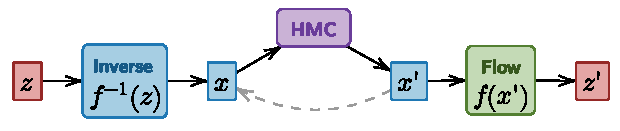
\includegraphics[width=\columnwidth]{assets/ftHMC}
      \caption{\label{fig:ftHMC}Normalizing Flow with inner HMC block.}
    \end{figure}
    %
    Our goal is to evaluate expectation values of the form
    %
    \begin{equation}
      \langle \mathcal{O}\rangle = \frac{1}{\mathcal{Z}}\int dx \,\mathcal{O}(x) e^{-S(x)}.
      \label{eq:expval}
    \end{equation}.
    %
    Using a normalizing flow, we can perform a change of variables \(x = f(z)\) so Eq.~\ref{eq:expval} becomes 
    %
    \begin{align}
      \langle \mathcal{O}\rangle 
        &= \frac{1}{\mathcal{Z}}\int dz\, |\det[J(z)]|\, \mathcal{O}(f(z))\,
        e^{-S(f(z))}, \quad\text{where}\quad J(z) = \frac{\partial f(z)}{\partial z} \\
        &= \frac{1}{\mathcal{Z}}\int dz \mathcal{O}(f(z)) e^{-S(f(z)) + \log|\det[J(z)]|}.
      \label{eq:expval_modified}
    \end{align}
    %
    The Jacobian matrix \(J(z)\) must satisfy
    %
    \begin{enumerate}
      \item Injective (1-to-1) between domains of integration
      \item Continuously differentiable (\emph{or}, differentiable with continuous inverse).
    \end{enumerate}
    %
    The function \(f\) is a \emph{trivializing map} when \(S(f(z)) - \log|\det J(z)| = \text{const.}\), and our
    expectation value simplifies to 
    %
    \begin{equation}
      \langle \mathcal{O}\rangle = \frac{1}{\mathcal{Z^{*}}}\int dz\, \mathcal{O}(f(z))\quad\text{where}\quad
      \frac{1}{\mathcal{Z^{*}}} = \frac{1}{\mathcal{Z}}\exp(-\mathrm{const}).
    \end{equation}
    %
  % \end{block}
  % \begin{block}{HMC with Normalizing Flow}
    % \heading{HMC with Normalizing Flows}
  \end{block}
  \begin{block}{HMC with Normalizing Flows}
    We can implement the trivializing map defined above using a normalizing flow model.
    %
    For conjugate momenta \(\pi\), we can write the Hamiltonian 
    \begin{equation}
      H(z, \pi) = \frac{1}{2}\pi^{2} + S(f(z)) - \log|\det J(f(z))|
    \end{equation}
    and the associated equations of motion as 
    \begin{align}
      \dot z &= \frac{\partial H}{\partial \pi} = \pi\\
        % \quad\text{and}\quad%
      \dot{\pi} &= -J(z)S'(f(z)) + \mathrm{tr}\left[J^{-1}\frac{d}{dz}J\right]
        % \dot{\pi} = -\frac{\partial H}{\partial z} = -J(z) S'(f(z)) - \log|\det J(z)|.
    \end{align}
    %
    If we introduce a change of variables \(\pi = J(z)\rho = J(f^{-1}(x))\rho\) and \(z = f^{-1}(x)\), the determinant
    of the Jacobian matrix reduces to \(1\) and we obtain the modified Hamiltonian
    %
    \begin{equation}
      \tilde H(x,\rho) = \frac{1}{2}\rho^{\dagger}\rho + S(x) - \log|\det J|.
    \end{equation}

    As shown in Fig.~\ref{fig:ftHMC}, we can use \(f^{-1}: z\rightarrow x \) to perform HMC updates on the transformed
    variables \(x\), and \(f: x\rightarrow z\) to recover the physical target distribution.

    % We can use the trained flow model together with the HMC algorithm by
    % performing the leapfrog updates in the
    % transformed space by first transforming our initial state,
    % x_{0} \xrightarrow[]{f} z_{0} \xrightarrow[]{\text{HMC}} z_{1} \xrightarrow[]{\text{HMC}} z_{2}%

    %%%%%%%%%%%%%%%%%%%%%%%%%%%%%%%%%%%%%%%%%%%%%%%%%%%
    % \begin{equation}
    %   f: x_{0}\rightarrow z_{0} \xrightarrow[]{\text{HMC}} z_{1} \xrightarrow[]{\text{HMC}} z_{2}%
    %   \rightarrow \ldots \rightarrow z_{N}
    % \end{equation}
    % and using the inverse to transform back to physical space, \(f^{-1}: z_{N}\rightarrow x_{N}\), as shown in
    % Figure~\ref{fig:ftHMC}.
    %%%%%%%%%%%%%%%%%%%%%%%%%%%%%%%%%%%%%%%%%%%%%%%%%%%
    % \begin{figure}
    %   \centering
    %   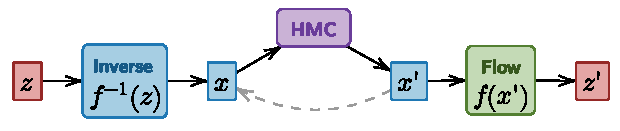
\includegraphics[width=\columnwidth]{assets/ftHMC}
    %   \caption{\label{fig:ftHMC}Normalizing Flow with inner HMC block.}
    % \end{figure}

  % \begin{alertblock}{Acknowledgements}
  \vspace{\baselineskip}
  \centering{\alert{\textbf{Acknowledgements}}}

    \begin{footnotesize}
      \alert{This research used resources of the Argonne Leadership Computing Facility, which is a DOE Office of Science User
      Facility supported under Contract DE-AC02-06CH11357.  This research was supported by the Exascale Computing
      Project (17-SC-20-SC), a collaborative effort of the U.S. Department of Energy Office of Science and the National
    Nuclear Security Administration.}
      % This research used resources of the Argonne Leadership Computing Facility, which is a DOE Office of Science User
      % Facility supported under Contract DE-AC02-06CH11357.  This research was supported by the Exascale Computing
      % Project (17-SC-20-SC), a collaborative effort of the U.S. Department of Energy Office of Science and the National
      % Nuclear Security Administration.  This work describes objective technical results and analysis. Any subjective
      % views or opinions that might be expressed in the work do not necessarily represent the views of the U.S.  DOE or
      % the United States Government.
  \end{footnotesize}
  % \end{alertblock}
  \end{block}


\end{column}

\separatorcolumn

\begin{column}{\colwidth}
  \begin{block}{2D U(1) Gauge Theory}
    \begin{wrapfigure}{l}{.25\columnwidth}
      \includegraphics[width=0.25\columnwidth]{assets/plaq.pdf}
      \caption{\label{fig:plaquette}Plaquette}%, \(P\)}
    \end{wrapfigure}
    Let \(U_{\mu}(n) = e^{i x_{\mu}(n)} \in U(1)\), with \(x_{\mu}(n) \in \left[-\pi, \pi\right]\) denote the \emph{link
    variables}, where \(x_{\mu}(n)\) is a link at the site \(n\) oriented in the direction \(\hat\mu\).

    We can write our target distribution, \(p(x)\), in terms of the Wilson action \(S(x)\) as
    %
    \begin{align}
      p(x)&\propto e^{- S(x)}, \quad \text{where}\quad S(x) \equiv \sum_{P} 1 - \cos x_{P}\quad\text{and}\\
      x_{P} &= x_{\mu}(n) + x_{\nu}(n+\hat{\mu})-x_{\mu}(n+\hat{\nu}) - x_{\nu}(n)
    \end{align}
    %
    as shown in Figure.~\ref{fig:plaquette}.
    %
    % \begin{equation}
    %   x_{P} = x_{\mu}(n) + x_{\nu}(n+\hat{\mu})-x_{\mu}(n+\hat{\nu}) - x_{\nu}(n)
    % \end{equation}
    %
    For a given lattice configuration, we can define the \emph{topological charge} \(Q \in \mathbb{Z}\) as
    %
    \begin{equation}
      Q = \frac{1}{2\pi}\sum_{P} \arg(x_{P}), \quad\text{where}\quad \arg(x_{P}) \in [-\pi,\pi].
    \end{equation}
    %
    We are interested in how this quantity evolves over a finite length Markov Chain, in particular we can define the
    \emph{tunneling rate}, \(dQ\) as
    \begin{equation}
      dQ = \sqrt{(Q_{i+1} - Q_{i})^2}
    \end{equation}
    where the difference is between subsequent states in the chain.
  \end{block}

  \begin{block}{Results}
    % \heading{HMC}
    \begin{figure}
      \begin{subfigure}{0.48\columnwidth}
        \centering
        \includegraphics[width=\columnwidth]{assets/hmc/dq_8x8_beta7_hmc_live1.png}
        \caption{\label{fig:hmc8beta7}\(8\times8\) lattice, HMC at \(\beta = 7\)}
      \end{subfigure}
      \begin{subfigure}{0.48\columnwidth}
        \centering
        \includegraphics[width=\columnwidth]{assets/hmc/dq_16x16_beta7_hmc_live.png}
        \caption{\label{fig:hmc16beta7}\(16\times16\) lattice, HMC at \(\beta = 7\)}
      \end{subfigure}
      \caption{Tunneling rate vs MC trajectory for HMC, demonstrating \emph{topological freezing} resulting in large
      integrated autocorrelation times.}
    \end{figure}
    \begin{figure}
      \begin{subfigure}{0.48\columnwidth}
        \centering
          \includegraphics[width=\columnwidth]{assets/fthmc/beta7/dq_8x8_beta7_fthmc_live1.png}
          \caption{\label{fig:fthmc8beta7}\(8\times8\) lattice, HMC \(+\) Normalizing Flow at \(\beta = 7\)}
      \end{subfigure}
      \begin{subfigure}{0.48\columnwidth}
        \centering
        \includegraphics[width=\columnwidth]{assets/fthmc/beta7/dq_16x16_beta7_fthmc_live.png}
        \caption{\label{fig:fthmc16beta7}\(16\times16\) lattice, HMC \(+\) Normalizing Flow at \(\beta = 7\)}
      \end{subfigure}
      \caption{Tunneling rate vs MC trajectory for HMC with trained Normalizing Flow, demonstrating an improved
      tunneling rate compared to HMC.}
    \end{figure}
  \end{block}
  %   \begin{table}
  %     \centering
  %     \begin{tabular}{l r r c}
  %       \toprule
  %       \textbf{First column} & \textbf{Second column} & \textbf{Third column} & \textbf{Fourth} \\
  %       \midrule
  %       Foo & 13.37 & 384,394 & $\alpha$ \\
  %       Bar & 2.17 & 1,392 & $\beta$ \\
  %       Baz & 3.14 & 83,742 & $\delta$ \\
  %       Qux & 7.59 & 974 & $\gamma$ \\
  %       \bottomrule
  %     \end{tabular}
  %     \caption{A table caption.}
  %   \end{table}
  \begin{block}{References}
    \nocite{*}
    \footnotesize{\bibliographystyle{plain}\bibliography{poster}}
  \end{block}
\end{column}
\separatorcolumn
\end{columns}
\end{frame}
\end{document}
